\documentclass[10pt,letterpaper]{article}
\usepackage[utf8]{inputenc}
\usepackage{graphicx}
\usepackage{rotating}
\bibliographystyle{ecology.bst}


\begin{document}
% Add line number
\linenumbers
\modulolinenumbers[1]

% Double space
\doublespacing

\section{Title:}\label{title}

\begin{itemize}
  \item Inferring species interactions from ecological data
  \item A quantitative comparison of methods for Inferring species interactions
  from ecological data
\item Comparing inferences for species interactions from ecological data
\item On the use of ecological data for comparing species interactions
\item Comparing methods for inferring species interactions
\item A statistical analysis of methods for inferring species interactions.
\item ?
\end{itemize}

\section{Authors*}\label{authors}

\begin{itemize}
  \item Ignasi Bartomeus
  \item Kevin Cazelles
  \item F. Guillaume Blanchet
  \item Mickaël Hedde
  \item Ignacio Morales Castilla
  \item Mathilde Besson
  \item David Beauchesne
  \item Dominique Gravel
  \item Timothée Poisot
  \item Ben Weinstein
  \item Steve Vissault
\end{itemize}

\emph{Current author order drawn from a multinomial distribution, which,
ironically, might be the only acceptable use case for this distribution in this
manuscript.}

\emph{Target Journals}: Methods in Ecology and Evolution, Ecological Monographs,
Annual Review of Ecology, Evolution, and Systematics.

\section{Introduction}\label{introduction}

Biotic interactions form the backbone of biodiversity
\cite{bascompte_plant-animal_2007}. Understanding the strength, direction, and
symmetry of species interactions provides insights into the maintenance of
assemblages and potential threats from anthropogenic change. Combined with
abiotic factors, biotic interactions constrain the distributions of species,
shape the evolution of phenotypes, and influence the stability of natural
systems \cite{schleuning_predicting_2015}. A common tool for understanding
interaction are ecological networks, in which each species (nodes) are connected
based on the strength and direction of interactions (links)(Jordano 1987).
Documenting and analyzing these networks is essential to understand the rules
underlying pairwise species interactions (Bascompte et al. 2006), quantifying
ecosystem functioning (Thomson et al 2012), and predicting the biodiversity
consequences due to anthropogenic change (ref).

Species traits are at the core of biological interactions (Bartomeus et al.
2016). In this paper, we defined traits as phenotypic adaptations to exploit abiotic or
biotic resources. We used traits as our principal mechanism to explain when
species can interact. The foremost requirement for species interactions is
species co-occurrence, which is itself driven by traits through environmental
filtering and local adaptation (Hillerislambers, Mayfield, but see Kraft). If
species co-occur, they may interact if their respective traits promote the
efficiency of resource extraction. In addition, traits can be represented by
phylogenetic information, in which evolution history constrains trait evolution
either directly through phylogenetic conservatism or indirectly through exposure
to similiar environmental conditions (Graham and Wiens 2005).

The traits promoting species co-occurrence and interaction may be hidden from
us, either through lack of sampling, or due to their complexity. In these cases,
the co-occurrence of species is used as a proxy for interaction. Given the
correlation in distribution or abundance of species across space or time,
co-occurrence based methods attempt to circumvent trait-based models by assuming
that species which consistently co-occur, and whose populations co-vary, may
have important biotic interactions. We therefore see co-occurrence based methods
as an extension of specific trait-based models when the mechanisms promoting
interactions are unknown or unobserved.

In spite of increasing efforts, it is unlikely that ecologists will empirically
document the enormous number of interactions existing in nature
(Morales-Castilla et al. 2015). Therefore, complementing field work with models
of species interactions is a promising avenue for understanding the complexity
of the natural world(ref). While direct inference will often be preferable, many
interactions are rare, infrequent, or impossible to detect by human observation.
Model-based inference for ecological networks provides three important aspects,
i) it establishes mechanistic relationships among species, ii) it estimates
uncertainty given empirical observation, and iii) it provides an avenue to
predict future interactions. We follow Poisot (2015) and Cazelles (2016) in
formulating our general conceptual model of species interactions (Fig. 1). There
is a pool of potential interactions, termed a metaweb, in which species could
interact based on co-occurrence. Any given observation we make is an attempt to
recover these relationships using empirical data. We use these data to fit a
model based on either species taxonomic identity or phenotypic characteristics.
This model can used to predict the interactions among observed species, given
the uncertainty due to spatial and temporal stochasticity of interactions, or a
new network, based on the presence of a novel species in the assemblage. From
these predictions, we can estimate structural network properties, such as
connectance and nestedness, while simultaneously propagating our uncertainty
throughout the analysis. In this paper, we review the methods proposed to build
models of species interactions, emphasizing each method's utility for predicting
the position of a novel species in the network.

From this conceptual framework, we can decide on a set of optimal criteria to
compare existing models. While there is unlikely to be any single method that
meets all our expectations, by defining a set of standards, we can more
transparently judge the relative merits of each method for our particular goal.
Our foremost goal is to generate a prediction of the links among co-occurring
species based on an estimated probability of interaction. This prediction should
come with a statement of uncertainty regarding our confidence in parameter
estimates based on empirical data. An ideal method will make reasonable
assumptions about the interdependence of observations, and be relatively
insensitive to low sampling effort. The mechanism determining the links among
species should be clear and grounded within ecological theory, such that we can
use our method to make a prediction about the placement of a new species in the
network based on a fitted model.

\subsection{Models of species
interactions}\label{models-of-species-interactions}

\subsubsection{Regression-based Models}\label{regression-based-models}

The simplest model of species interactions is

eq i.

\[Y_{i,j} = \rho_{i,j}\] Where the probability of interaction among species i
and species j is a fixed value (\(\rho_{i,j}\)). Using empirical data, we might
try to estimate this value by dividing the number of observations by the total
number of observations for any pair of species. While this is straightforward,
why might it be insufficient? Foremost, it contains no estimate of uncertainty.
The estimate is given without any consideration for the variance due to
sampling, spatial or temporal stochasticity. To add uncertainty, we draw our
observations from a statistical distribution.

eq ii.

\[ Y_{i,j} \sim Bernoulli(\rho_{i,j}) \]

We can now estimate the probability of interaction, as well as the uncertainty
based on sampling stochasticity. Yet this model is still unsatisfying. It is
non-mechanistic, it depends wholly on species identity, and uses no ecological
theory or inference. Therefore, it is difficult to ascribe meaning to a set of
interactions, or understand how they might change in the future. We cannot use
the inferences from data to make a prediction about a new species not in
dataset.

To make our model more useful, we might add a covariate, such that

eq. iii

\[ Y_{i,j} \sim Bernoulli(\rho_{i,j})\] \[ logit(\rho_{i,j}) = \alpha_{i,j} +
\beta_{i,j} * x_{i,j} \]

In which a link between species i and j is a Bernoulli trial with a probability
of success \(\rho_{i,j}\). The probability of success will vary based on some
ecological principle (\(x_{i,j}\)), for example, the similarity in functional
traits among species i and j:

eq. V

\[x_{i,j}= f(Trait_i,Trait_j)\]

A variety of trait-matching functions may be biologically plausible. For
example, the absolute value of the difference between traits (e.g. \(|trait_i -
trait_j|\)) or a binary difference (e.g. \(trait_i > trait_j\)), could be used
to predict which species may interact. Alternatively, the covariate may
represent the phylogenetic relatedness of species, or their relative response to
a given environmental variable.In some cases, we cannot provide a simple
trait-matching function (eg V), but must use a statistical tool to infer the
best possible combination of traits among co-occurring species that predicts
interactions. Machine learning tools provide an ideal compliment to traditional
linear models when we cannot anticipate the combinations of traits that can
influence species interaction rates. Unsupervised learning tools, such as random
forests, can give us the associations among species given a set of complex
traits. Regardless of the exact form of regression, this framework satisfies two
important goals: it allows for estimates of uncertainty in species interactions,
and it provides a mechanism shaping the probability of an interaction.

So far, we have only captured the uncertainty in the process model, the inherent
temporal or spatial stochasticity in our ecological process of interest (Hooten
and Hobbs). We may need to also account for the uncertainty in the observation
model, the ability to detect interactions given that they occur. The separation
of the observation and process model translates our ecological mechanism into
specific predictions about empirical data. For binary networks, one
straightforward way to account for the observation of interactions is to model
the detectability of network interactions.

eq iv.

\[ Y_{i,j,k} \sim Bernoulli(\phi_{i,j})\] \[ \phi_{i,j} = \omega_{i,j} *
z_{i,j}\] \[z_{i,j} \sim Bernoulii(\rho_{i,j})\] \[ logit(\rho_{i,j}) =
\alpha_{i,j} + \beta_{i,j} * x \]

Where the observation of a link between species i and species j at time k is a
Bernoulli trial with a probability \(\phi_{i,j}\), which is the outcome of the
detectability of an interaction (\(\omega_{i,j}\)) and the latent state
(\(z_{i,j}\)). This latent state is the true, but unobserved, existence of a
link, as predicted by our ecological mechanism of interest (see eq IV). Our
ability to detect this latent state depends on the detectability of an
interaction (\(\omega_{i,j}\)). The benefit of this approach is that
differentiates the probability of detection from the probability of occurrence.
Importantly, because we have explicitly defined some temporal window (k),
interactions with different levels of sampling effort can be directly compared.

\subsubsection{Logic-based methods}\label{logic-based-methods}

{[}Ben Weinstein: For someone to fill in.{]}

\subsubsection{Occurrence-based methods}\label{occurrence-based-methods}

{[}Ben Weinstein: For someone to fill in.{]}

\subsubsection{Non-parametric methods}\label{non-parametric-methods}

The above methods are model based, that is, they largely use parametric
distributions to estimate the liklihood of the data given estimated model
parameters. An alternative approach is to use multivariate statistics to create
association matrices. One such method is called fourth-corner analysis, which is
a type of three table ordination (sometimes called `RLQ' analysis) (Doledec
1996). In bipartite networks, fourth-corner analysis relates the matrix of
species interactions to a matrix of traits from one level (e.g.~plants) to
another level (e.g.~pollinators) via the matrix of species innteractions (Dray \&
Legendre, 2008). This produces a correlation matrix, which is then compared to a
null expectation through matrix randomization. Randomization is a familiar tool
in network ecology, in which permuatation rules are used to compare the observed
test statistic (e.g the correlation among species occurrences) to a null
distribution based on some matrix constraint. Common constraints include the
mantainance of row sums, column sums, or other all marginal values, such that
only the identity of partners are switched. After each permutation, the test
statistic is recalulcating, yielding a null distribution. By comparing whether
the observed test statistic falls within the upper or lower 5th quantile of the
null distribution, studies distinguish whether their results could have been
generated at random given their sampling effort.

\section{Methods}\label{methods}

Our goal is provide a conceptual framework for the broad array of potential
methods described above. Our three criteria for qualitative comparison are: 1)
Can the method account for the uncertainty in species observations?, 2) Does it
provide an ecological mechanism to infer the probability of species
interactions, and 3) Can it be used to predict an novel interaction? In addition
to qualitative comparison, we provide a quantitative analysis of methods for
inferring species interactions. From a quantitative perspective, we are
interested in methods which accurately reflect true relationships among data,
are relatively insensitive to sampling effort, and make reasonable assumptions
about the interdependence of species observations. We use a combination of
simulated and empirical data to establish a benchmark dataset to compare the
accuracy and sensitivity of currently proposed methods.

\section{Quantitative comparisons}\label{quantitative-comparisons}

-\textgreater{} results: - cross comparison \textbar{} real and simulated data -
-sensitivity \textbar{} - interpretation of probabilities - method description
-for comparison

\section{Results}\label{results}

\section{Discussion}\label{discussion}

\subsection{Perspectives}\label{perspectives}

\begin{itemize} \item guidelines \item challenges \item next steps \end{itemize}

\subsection{On the virtue of prediction of species
interactions.}\label{on-the-virtue-of-prediction-of-species-interactions.}

In a context where novel ecosystems arise as a result of species invasions or
due to geographic shifts tracking climate change, our ability to predict future
interactions will limit how efficiently we anticipate and respond to threats on
biodiversity (i.e.~species local extinctions) and on humans (i.e.~spread of
infectious disease or plagues affecting to crops).

\emph{{[}Ben Weinstein: Previous text from Nacho:{]}} Indeed, on the quest for
describing species interactions, traits had played a pivotal role and several
methods have recently emerged to test hypotheses of trait matching for pairwise
interactions (Stang et al 2006, Dehling et al. 2014, Bartomeus et al 2016) or
understand the phylogenetic structure of ecological networks (Rezende et al.
2007). However, generating biological meaningful predictions of species
interactions and its emerging properties have proven challenging (Olito and Fox
2014). An ideal method is grounded in ecological theory, which makes the
description of ecological interactions interpretable. This method should be able
to not only describe, but also predict ecological interactions based on a set of
simple parameters. Importantly, this predictions should be accompanied by an
associated uncertainty. In addition, given the difficulty of empirically
assessing complete interaction networks, this method should be also robust to
the use of incomplete data. There is an urgent need to better understand how
communities interact and predict new interactions which will inevitably occur as
a result of human induced rapid environmental change. In addition, our
understanding of how species interact is limited to the few interactions are
directly observable such as pollination of predation, but key species
interactions not directly observable remains unlocked. Interactions inferences
may be the only option for describing and predicting interactions in soil food
webs or bacteria-phage networks. Finally, traits also relate to the fitness
effects gained by both interaction partners. This can potentially establish a
link with to modern coexistence theory. In fact, neutral expectations
postulating that species abundances are the main drivers of interactions, are
not incompatible with the underlying role of species traits shaping species
abundances via effects in fitness (Bartomeus et al. 2016).

\section{Literature cited}\label{literature-cited}

\bibliography{referencesNew}

\section{Boxes}\label{potential-boxes}

\subsection{Soil ecology}\label{soil-ecology}

\subsection{Climate changes and alien
species}\label{climate-changes-and-alien-species}

\subsection{Community/evolution ecology}\label{communityevolution-ecology}

\begin{figure}
  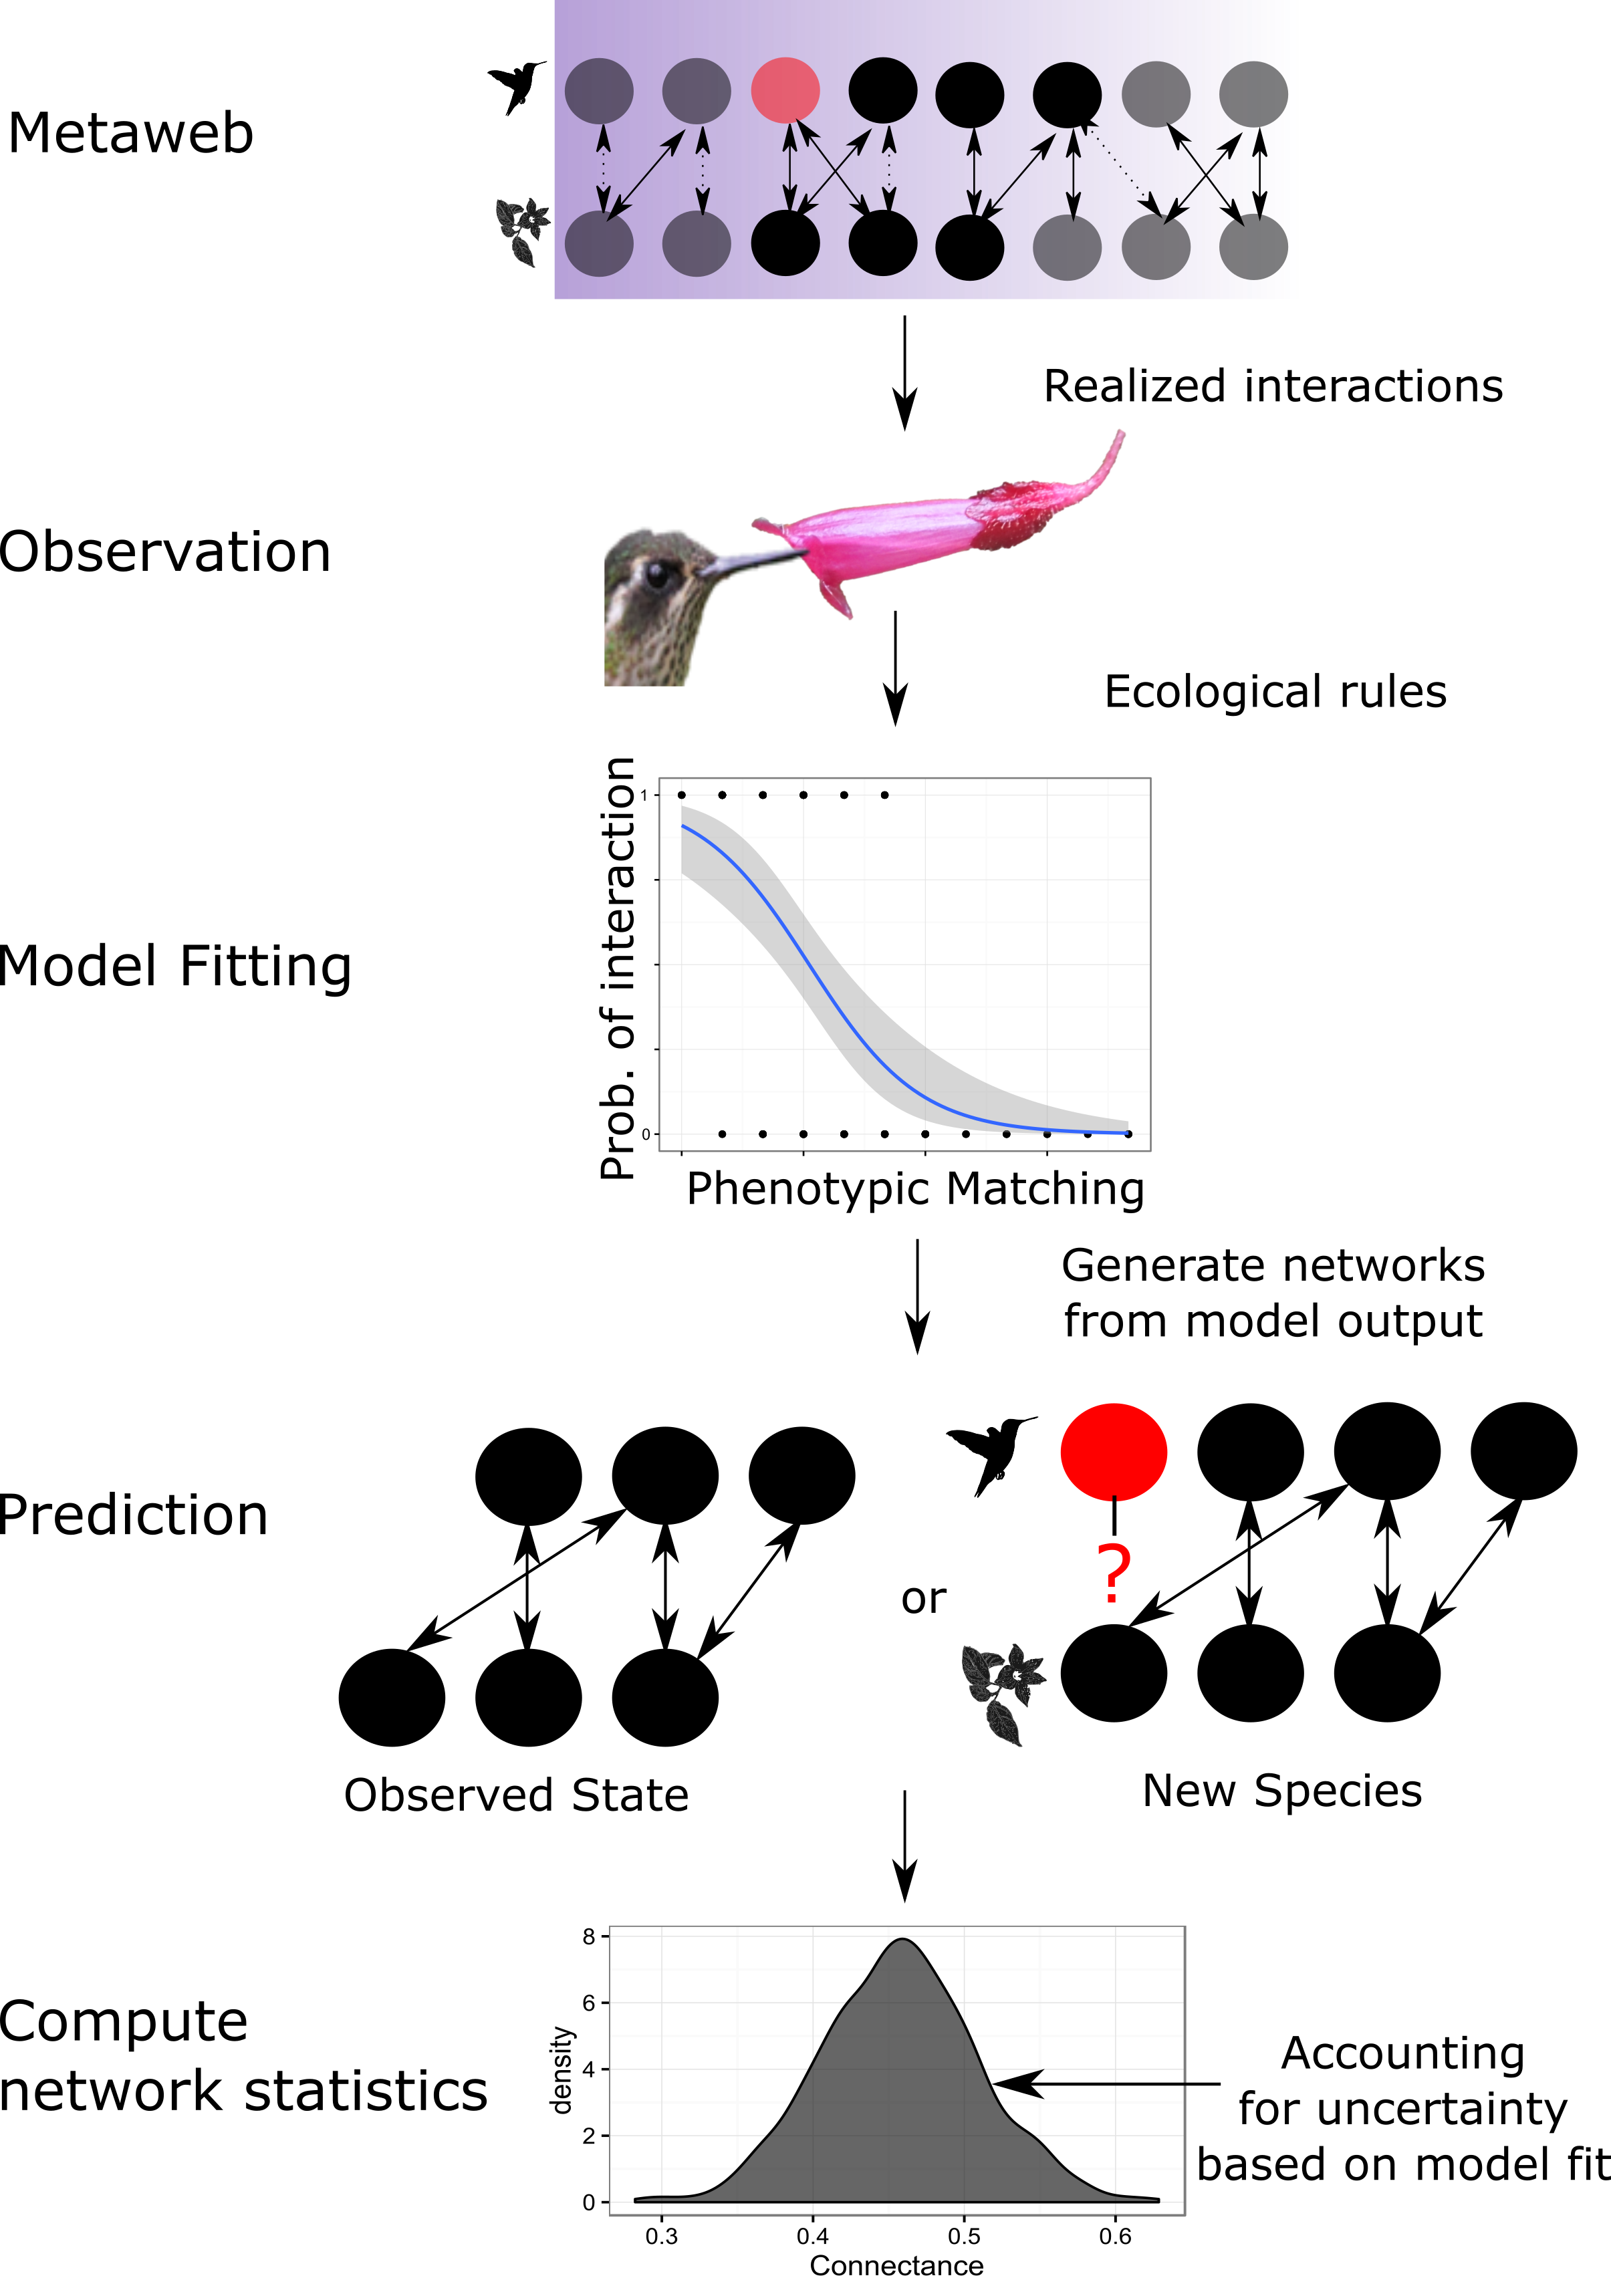
\includegraphics[width=\linewidth]{Figures/ConceptualFigure.png}
  \caption{Conceptual outline of using models to estimate species
  interactions}
  \label{fig:concept}
\end{figure}


\begin{sidewaystable}
\centering
\caption{Methods compared and how they apply}
\label{comparisonTab}
\begin{tabular}{llccccccccccc}
                                                & \multicolumn{5}{c}{Input Data}                                                                                                                                         & \multicolumn{1}{c}{}              & \multicolumn{1}{c}{}              & \multicolumn{1}{c}{}           & \multicolumn{1}{c}{}       & \multicolumn{1}{c}{}                   & \multicolumn{1}{c}{}                                                                                                                     \\
                                                & \multicolumn{1}{c}{abundance} & \multicolumn{1}{c}{Indirect  knowledge} & \multicolumn{1}{c}{Co-occurence} & \multicolumn{1}{c}{Trait} & \multicolumn{1}{c}{Phylogeny} & \multicolumn{1}{c}{Theory-driven} & \multicolumn{1}{c}{Type of links} & \multicolumn{1}{c}{Predictive} & \multicolumn{1}{c}{Output} & \multicolumn{1}{c}{Hypothesis testing} & \multicolumn{1}{c}{Example}                                                                                                              \\
Fourth-corner                                   & x                             &                                         &                                  & x                         &                               & yes                               & quantitative                      & mecanistic                     &                            &                                        & \begin{tabular}[c]{@{}l@{}}I\_eat (Beauschene et al. 2016)\\ Markov logic, Intuitive Logic Programming (Vacher et al. 2016)\end{tabular} \\
Maching learning                                & x                             & x                                       & (x)                              & (x)                       & (x)                           & no                                & quantitative                      & data-based                     &                            &                                        & Rohr et al. 2014, Rohr et al. 2016                                                                                                       \\
Direct mathcing-centrality                      &                               &                                         &                                  & x                         & x                             & yes                               & quantitative                      & mecanistic                     &                            &                                        &                                                                                                                                          \\
Indirect matching-centrality                    &                               &                                         &                                  &                           &                               &                                   &                                   &                                &                            &                                        &                                                                                                                                          \\
Niche model                                     &                               &                                         &                                  &                           &                               &                                   &                                   &                                &                            &                                        &                                                                                                                                          \\
Hierarchical model                              &                               &                                         &                                  &                           &                               &                                   &                                   &                                &                            &                                        &                                                                                                                                          \\
Null model                                      &                               &                                         &                                  &                           &                               &                                   &                                   &                                &                            &                                        &                                                                                                                                          \\
Joint Spatial Division and Multiplexing (JSDM)  &                               &                                         &                                  &                           &                               &                                   &                                   &                                &                            &                                        &                                                                                                                                          \\
Intercept                                       &                               &                                         &                                  &                           &                               &                                   &                                   &                                &                            &                                        &                                                                                                                                          \\
GLM/cooccur                                     &                               &                                         &                                  &                           &                               &                                   &                                   &                                &                            &                                        &                                                                                                                                          \\
Grouping species into nodes (functional groups) &                               & x                                       &                                  & x                         &                               & no                                & Binary (quantitative)             & no                             &                            &                                        &                                                                                                                                          \\
Expert-based assesment of links                 &                               & x                                       &                                  & x                         &                               & no                                & Binary (quantitative)             & no                             &                            &                                        &
\end{tabular}
\end{sidewaystable}



\end{document}
